% The sample PDF of PollisDatasets, for the PDF Files panel of Pollis: sections and subsections of
% placeholder text (lipsum) and a figure on page 1, Table 1 on page 2, notes on page 3.
% Table 1 is read from table1.csv (one line per row, cells separated by semicolons), and the same
% file is attached to the PDF, so an extracted table can be checked against the values typeset.
% To make a test PDF of your own, edit table1.csv or this file, typeset it with
% PollisTeX.compile("sample.tex"), and attach table1.csv with Poppler's pdfattach.
\documentclass[11pt]{article}
\usepackage[a4paper, margin=2.5cm]{geometry}
\usepackage{graphicx}
\usepackage{float}
\usepackage{booktabs}
\usepackage{csvsimple}
\usepackage{lipsum}
\usepackage[hidelinks]{hyperref}
\hypersetup{pdftitle={Returns to Schooling: A Sample Report}, pdfauthor={PollisDatasets}, pdfsubject={A sample PDF for the PDF Files panel of Pollis}, pdfkeywords={sample, table, PDF}}

\title{Returns to Schooling: A Sample Report}
\author{PollisDatasets}
\date{}

\begin{document}

\maketitle

\section{Introduction}

\lipsum[1]

\subsection{Data}

\lipsum[2]

\begin{figure}[H]
\centering
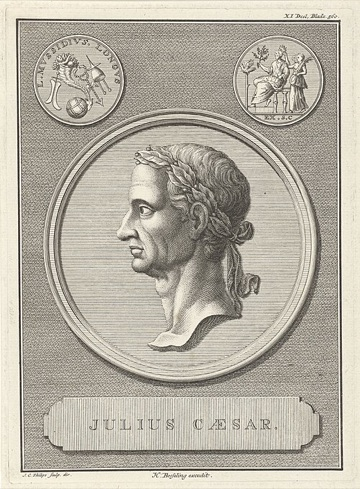
\includegraphics[width=4.5cm]{caesar.jpg}
\caption{Gaius Iulius Caesar, aere incisus a Iohanne Caspare Philips, MDCCXLV.}
\end{figure}

\newpage

\section{Results}

\lipsum[3][1-3]

\begin{table}[H]
\centering
\caption{Log hourly wage on schooling and experience}
\begin{tabular}{lrr}
\toprule
\csvreader[no head, separator=semicolon, late after line=\\, late after first line=\\\midrule, late after last line=\\\bottomrule]{table1.csv}{}{\csvcoli & \csvcolii & \csvcoliii}
\end{tabular}

\medskip
{\footnotesize Standard errors in parentheses. *** p$<$0.01, ** p$<$0.05, * p$<$0.1}
\end{table}

\newpage

\section{Notes}

\subsection{About Table 1}

The numbers in Table 1 are made up for this example, and its cells are attached to this file as \texttt{table1.csv}.

\subsection{Sed ut perspiciatis}

\lipsum[4]

\end{document}
